\documentclass[a4paper]{scrartcl}

%\usepackage[applemac]{inputenc}
\usepackage[utf8]{inputenc}
%\usepackage{a4wide}
\usepackage{graphicx}
\usepackage{tabularx}
\usepackage{pstricks-add}
\usepackage{url}
\usepackage{auto-pst-pdf}
\usepackage[english]{babel}

% Kopf- und Fusszeilen
\usepackage{fancyhdr}
\pagestyle{fancy}
\fancyhead{}
\fancyfoot{}
\lhead{HSR University of Applied Science Rapperswil}
\rhead{Term Project}
\lfoot{\copyright \ Nicolas Bigler, Michael Fisler}
\rfoot{Page \thepage}
\renewcommand{\headrulewidth}{0.4pt} 
\renewcommand{\footrulewidth}{0.4pt}


\title{
	\vspace{-30mm}
	\hspace{-40mm}
	
\includegraphics{Bilder/HSR_Logo_CMYK.eps}
	\newline
	\newline
	\newline
	\newline
	\newline
	\newline
	\newline
%\fbox{\textwidth}{
Validation of the Background Radiation Detector
%}
 \\ \ \\ Term Project \\ \ \\ \ }
\subtitle{
	Department of Computer Science \\ University of Applied Science Rapperswil \\ \ \\ \ Fall Term 2011\\ \ \\ \ \\ \ \\ \ \\ \ \\ \ 
}

\author{
Authors: Nicolas Bigler, Michael Fisler  \and
Advisor: Prof. Eduard Glatz \and		
Project Partner: - \and
External Co-Examiner: ? \and
Internal Co-Examiner: ?
}

%Suppress Date on Title Page
\date{}

% Absatzeinzug aufheben
\parindent 0pt

% Set Paragraph Spacing
\parskip 6pt

\begin{document}

%Marginals on the left Side 
\reversemarginpar
\maketitle
\newpage
\tableofcontents
\newpage
\listoffigures
\newpage
\listoftables
\newpage

\section{Task}
A \marginpar{Starting position} substantial part of the internet's traffic stems from misconfiguration, worms, malware, viral activity or all sorts of attacks and therefore is undesirable. As this kind of traffic is constantly present it often is referred to as ``internet background radiation''. The monitoring of the background radiation yields valuable information in terms of malicious activity and may be used to predict future trends.

At ETH Zurich a tool was developed to distinguish between one-way and two-way flows and subsequently classify one-way traffic using a set of predefined rules.

Until now the available data was limited since only packet headers were recorded. It was therefore difficult to successfully validate the Background Radiation Detector due to the lack of information.

To gain more Information a special infrastructure was set up at HSR to record the entire traffic within a five day span in order to enable a more thorough validation. In addition to the packet headers and flow data the new infrastructure provides payloads from one-way flows and intrusion detection system (IDS) alerts.

Through\marginpar{Mission} analysis of the collected data skillfully using and combining different analysis methods the rules used by the detector shall be validated and optimized. As far as possible the validation shall be automated. The goal is to determine the false negative (FN) and false positive (FP) rates for each class.
The methods to use are as follows:
\begin{itemize}
	\item analysis of the state sequence (flag sequence, TCP packets only)
	\item analysis of the network management information data (ICMP packet analysis)
	\item correlation of IDS alerts and flow data
\end{itemize}

The main focus of this validation is on the classes ``malicious scanning'' (rule 5), ``suspicious other'' (rules 6 to 8), ``backscatter'' (rules 9 to 11) and ``suspected benign'' (rule 15). Class ``Bogon'' needs no validation.

The original text of the task (in German) is enclosed in the appendix [ref?].
\newpage

\section{Abstract}

\section{Management Summary}
The\marginpar{Starting position} goal of this project is the validation of the ``Background Radiation Detector'' which was developed at ETH Zurich. In a first step the detector identifies one-way flows and in a second step classifies those flows using predefined rules. In order to validate these rules and if necessary adapt them packet and flow data was recorded in a five day period. Aditionally an intrusion detection system has been set-up to further investigate the cause of all incoming traffic.

Since\marginpar{Approach} we are dealing with very large PCAP files loading an entire file in Wireshark takes at least half an hour. In order to reduce the file size and thus allowing a more efficient manual analysis one-way flows from the original PCAP traces were written into new files according to the class they belong to.


blub \marginpar{Results} blub

blub \marginpar{Outlook} blub

\section{Technical Report}

\subsection{Infrstructure}
Data was collected between ... and ... on a server (``Collector'') connected between HSR's gateway and firewall.  The ``Collector'' is equipped with a high performance DAG Endace network card which allows to capture all packets even at full line rate. Using external time references the captured packet's timestamps are highly accurate. \cite{endace}. Attached to the collecting server a second server (``Analyzer'') is used to process and evaluate the data captured. It hosts an environment to compile and run validation software and tools such as Wireshark for further analysis.
\begin{figure}[ht]
	\begin{center}
		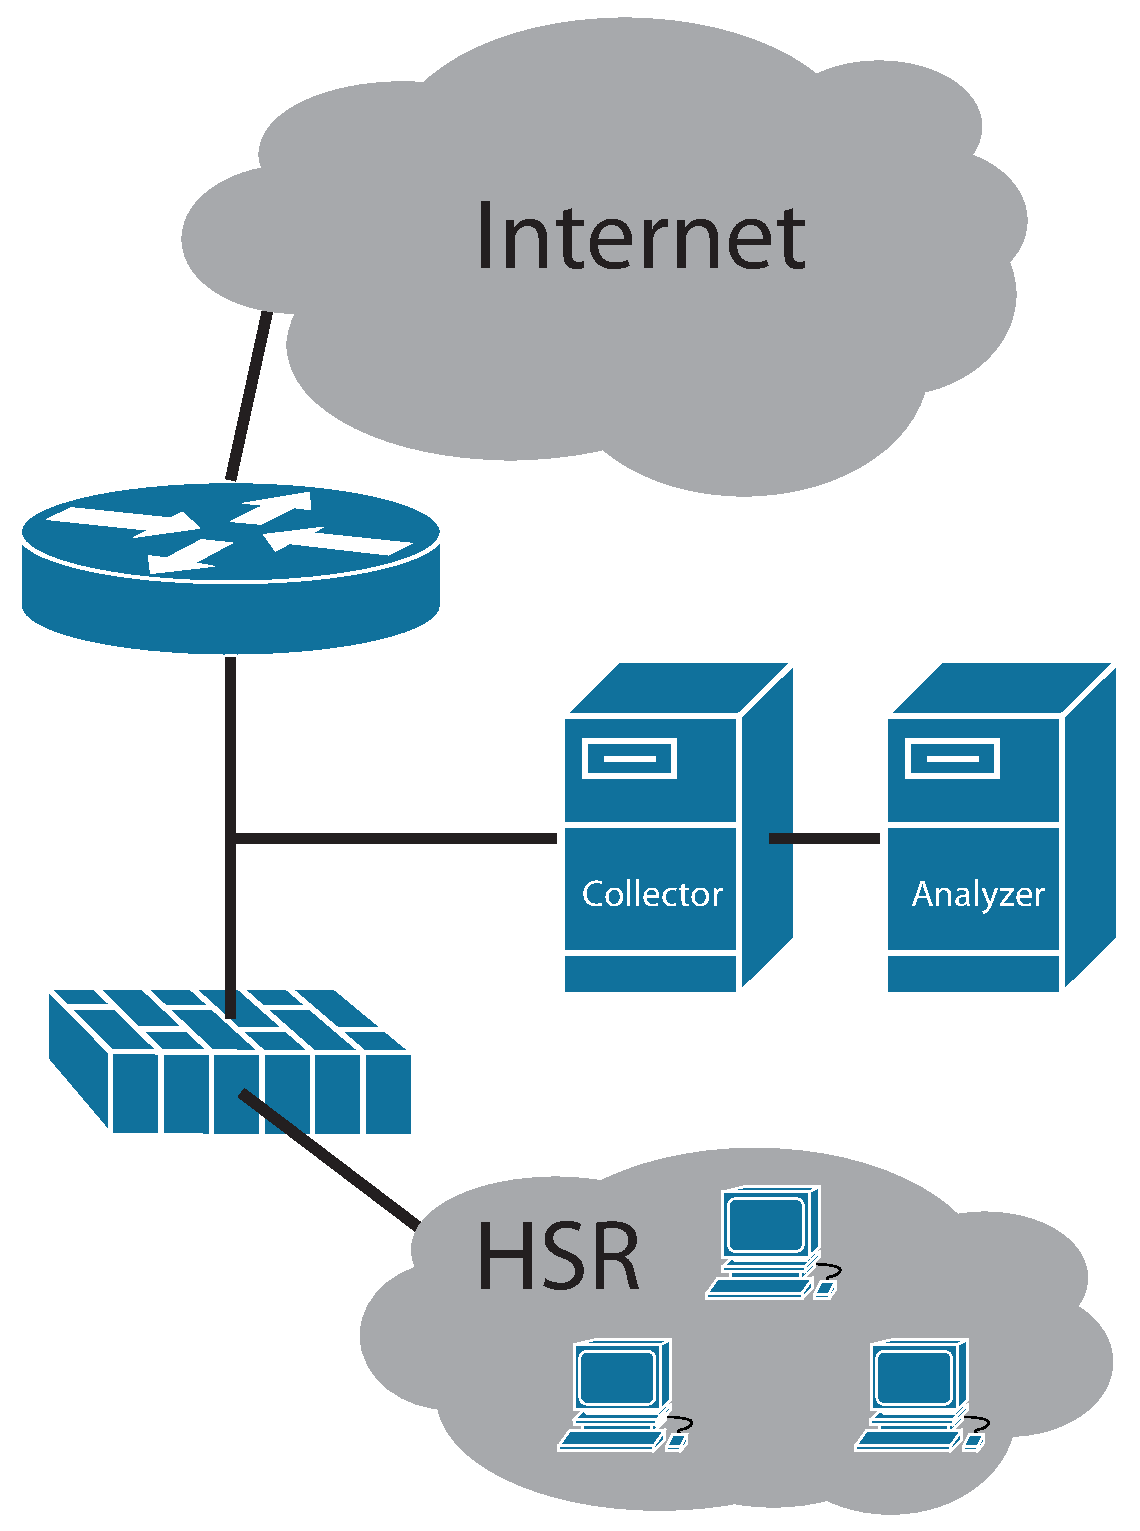
\includegraphics[width=200pt, keepaspectratio=true]{Bilder/Infrastruktur.eps}
		\caption{Validation infrastructure}
		\label{infra}
	\end{center}
\end{figure}

\subsection{Data}
The\marginpar{PCAP} validation is primarily based on PCAP traces which contain the entire traffic from and to the HSR in a five day span. The traces are split into one hour intervals. HSR is connected to the Switch network which doesn't filter traffic. We therefore get a good sample of the internet background radiation [quote Prof. Glatz].

Flow \marginpar{Flow data} data was generated from the PCAP files with YAF \cite{yaf} and converted from IPFIX to CFlow format. The resulting files contain flow data in 10 minute intervals. Each flow is defined by its starting time, its duration (which may exceed 10 minutes), the IP data and the flow direction. Only incoming flows (infl) and incoming flows which have a corresponding two-way flow with the same IP addresses and ports (q\_infl) are relevant for our validation.

Based\marginpar{Sign sets} on the flow data  Flow Daten wurden anschliessend mit dem O/W Classifier [] den verschiedenen Klassen zugeordnet. Als Resultat liegen Signdaten vor in denen die Klassenzugehörigkeit der Flows gespeichert ist.

In\marginpar{IDS alerts} addition to the flow and sign data, alerts generated by the open-source intrusion detection system Snort can be used to investigate the intent of the flows. In order to be able to correlate these alerts with the packet and flow data, the same anonymizing scheme was used.

\subsubsection{Data privacy}
In order to meet the data privacy requirements at HSR all IP addresses are anonymized and all data above the transport layer has been stripped from packets belonging to two-way flows. Layer 4 PDU are available for one-way flows only. The anonymization generates random IP addresses but preserves prefixes (i.e. subnet membership is preserved). It therefore is impossible to identify the hosts, networks oder services behind those IP addresses. As a consequence it is very difficult to figure out if a certain host is a regular server and neither the geographic location, nor the provider who owns the respective IP address can be identified. We discovered that the IP addresses 152.103.xxx.xxx are HSR addresses since they were present in almost all packets.

\subsubsection{Limitations of our flow data}
YAF has some limitations in terms of flow defragmentation. If a connection is terminated with a FIN flag and packets are retransmitted after that, YAF interprets those retransmissions as independent one-way flows. The same holds true if Multiple RST packets are sent. HOW MANY?

\subsection{Basic Validation Concepts}
In\marginpar{TCP} case of TCP one-way flows the only valid flag sequence is a sequence of multiple SYN flags. If only one SYN flag is sent we consider that to be a SYN scan because benign applications should try to establish a connection more than once if they don't receive a SYN/ACK. Most applicaitons use the default socket and therefore do that by default [quote Prof. Glatz]. Before a connection is established RFC 793 \cite{rfc_tcp} forbids the use of flags other than SYN. 

To\marginpar{UDP} validate UDP flows we use the UDP PDU's size. Packets without a payload are a priori suspicious. Regular UDP packets should at least contain protocol headers from OSI layers 5 to 7 even if no user data is sent and therefore contain a UDP PDU.
In addition to the existence of a PDU the variance of size over all packets within the flow may be used to identify malicious intent. If all PDUs are the same size the flow is certainly not a regular benign flow but rather a scan. BRINGT DIESES KRITERIUM ETWAS? AUSWERTUNG ANSCHAUEN!!!

\subsection{Flow Classes}
Im Folgenden wird die von der ``Background Radiation Detection''-Software verwendete Klassifizierung kurz erläutert und die Charakteristiken der einzelnen Klassen aus Sicht der Validierung aufgezeigt. Die Klassen sind disjunkt, so dass die jeweiligen False Positive und False Negative Raten theoretisch berechnet werden können unter der Voraussetzung, dass die einzelnen Flowdaten korrekt den Klassen zugeordnet werden können. Neben den Regeln zur Klassifizierung werden die Überlegungen und die daraus resultierenden Kriterien und Ansätze für die Validierung erläutert. Es werden bei den Regeln jeweils nur die für die Validation relevanten Kriterien angeführt, die restlichen sind in der Publikation von Prof. Eduard Glatz [] im Detail beschrieben.

\begin{figure}[ht]
\begin{center}
\psset{framesep=1.1pt,unit=1.1cm}
\begin{pspicture}(-5.1,-5.1)(5.1,5.1)
	\degrees[100]
	\pswedge[fillstyle=hlines,fillcolor=gray,hatchcolor=gray]{5}{ 0 }{65.24 }
	\rput(4.2; 32.62 ){\psframebox*{\small 65.24 \%}}
	\uput{5.2}[ 32.62 ](0;0){\small Malicious Scanning}
	\pswedge[fillstyle=hlines,fillcolor=gray,hatchcolor=gray]{5}{65.24 }{93.16 }
	\rput(4.2;79 ){\psframebox*{\small 27.92 \%}}
	\uput{5.2}[79 ](0;0){\small Suspicious Other}
	\pswedge[fillstyle=hlines,fillcolor=gray,hatchcolor=gray]{5}{93.16 }{95.39 }
	\rput(4.2;94.2 ){\psframebox*{\small 2.23 \%}}
	\uput{5.2}[94.2 ](0;0){\small Backscatter}
	\pswedge[fillstyle=solid,fillcolor=white,hatchcolor=white]{5}{95.39 }{95.52 }
%	\rput(4.2;95.4 ){\psframebox*{\small 0.13 \%}}
	\uput{5.2}[95.4 ](0;0){\small Serv. Unreach. (0.13 \%)}
	\pswedge[fillstyle=solid,fillcolor=white,hatchcolor=white]{5}{95.52 }{98.49 }
	\rput(4.2;97 ){\psframebox*{\small 2.97 \%}}
	\uput{5.2}[97 ](0;0){\small P2P Scanning}
	\pswedge[fillstyle=solid,fillcolor=white,hatchcolor=white]{5}{98.49 }{98.68 }
%	\rput(4.2;98 ){\psframebox*{\small 0.19 \%}}
	\uput{5.2}[98 ](0;0){\small Susp. Benign (0.19 \%)}
	\pswedge[fillstyle=solid,fillcolor=gray,hatchcolor=gray]{5}{98.68 }{98.94 }
%	\rput(4.2;98.7 ){\psframebox*{\small 0.26 \%}}
	\uput{5.2}[98.7 ](0;0){\small Bogon (0.26 \%)}
	\pswedge[fillstyle=solid,fillcolor=gray,hatchcolor=gray]{5}{98.94 }{100 }
	\rput(4.2;99.5 ){\psframebox*{\small 1.8 \%}}
	\uput{5.2}[99.5 ](0;0){\small Other}
\end{pspicture}
\caption{Die Klassen und ihre Häufigkeiten gemäss der Klassifizierung durch den ``O/W Classifier''. Insgesamt sind 95.93\% der Flows als bösartig (schraffiert), 3.29\% gutartig (weiss), 2.06\% nicht definiert (grau) eingestuft worden.}
		\label{class}
	\end{center}
\end{figure}

\subsubsection{Malicious Scanning}
Für\marginpar{Regeln} die Klasse ``Malicious Scanning'' gibt es drei Regeln: 

In\marginpar{Charakteris\-tika} dieser Klasse befinden sich alle bösartigen Scanaktivitäten. Mit Ausnahme des SYN Scans ist die Länge der Flows grundsätzlich nicht beschränkt. Es ist durchaus denkbar, dass mehrere Pakete unterschiedlicher Scanart in einem einzelnen Flow enthalten sein können. UDP Scans haben in der Regel einen spezifischen Payload, der von dem Zielservice abhängt \cite{nmap09}.

Für\marginpar{Validierung} die Validierung der TCP Flows werden die von NMAP vewendeten Scanmuster \cite{nmap09} verwendet:
\begin{itemize}
	\item Christmas Scan: Beim Christmas Scan wird ein Paket mit gesetzten FIN, PSH und URG Flags geschickt.
	\item Null Scan: Ein Paket ohne gesetzte Flags wird ohne vorhergehenden TCP-Verbindungsaufbau verschickt. 
	\item FIN Scan: Ein Paket mit gesetzten FIN-Flag wird ohne vorhergehenden TCP-Verbindungsaufbau geschickt.
	\item SYN Scan: Ein einzelnes Paket mit gesetztem SYN-Flag wird geschickt
\end{itemize}
Mit den oben aufgeführten Kriterien kann die True Positive Rate bestimmt werden. 
Für das Bestimmen der False Positive Rate wurden die nicht eindeutig als Scan verifizierten TCP-Flows manuell auf die Klassenzugehörigkeit überprüft.

Für die Analyse der ICMP Flows nutzen wir die Tatsache, dass Scanning nur mit ICMP Requests möglich ist, da alle anderen ICMP Arten nicht quittiert werden \cite{rfc_icmp}. Die False Positive Rate ergibt sich bei den ICMP Paketen folglich aus der Anzahl der ICMP Responses.

\subsubsection{Suspicious Other}
In\marginpar{Charakteris\-tika} dieser Klasse befinden sich alle Flows, die nicht den restlichen bösartigen Klassen ``Malicious Scanning'' und ``Backscatter'' zugewiesen werden können, aber vermutlich bösartigen Ursprungs sind. 

Alle\marginpar{Validierung} TCP Flows die keine gültige Flag-Sequenz aufweisen sind a priori als bösartig einzustufen. Falls eine gültige Flag-Srequenz vorliegt kann ohne Zusatzinformationen keine Zuordnung gemacht werden, da zum Beispiel bösartige Scans zur Tarnung auch gültige Sequenzen verwenden können \cite{nmap09}.

\subsubsection{Backscatter}
Unter\marginpar{Charakteris\-tika} Backscatter versteht man den eingehenden Verkehr, der durch Angriffe auf Rechner in anderen Netzen mit gefälschten Absenderadressen verursacht wird []. 

Durch\marginpar{Validierung} Backscatter ausgelöste ICMP Pakete können nur Replys sein, denn Backscatter ist immer eine Reaktion auf eingehende Pakete. Allfällige Requests fallen somit in die Kategorie False Positive.

Bei TCP dürfen keine SYN Flags vorkommen, da diese einen aktiven Verbindungsaufbau einleiten und somit nicht Backscatter sein können. Die Flag-Sequenzen in der Klasse Backscatter müssen gemäss der TCP-State Machine gültig sein weil der Ursprung der Pakete reguläre Hosts und Netzwerkgeräte sind. <-- UMSETZEN!

\subsubsection{Service Unreachable}
Unter\marginpar{Charakteris\-tika} Service Unreachable fallen alle Flows, die aufgrund eines temporär nicht verfügbaren Services entstehen.

Ein\marginpar{Validierung} Ansatz zur Validierung besteht darin, zu überprüfen ob sich die Zieladresse im von der HSR ungenutzten Adressraum befindet. Ist dies der Fall, liegt 

Da\cite{rfc_icmp} die HSR ausgehende ICMP Destination Unreachable Pakete nicht unterdrückt, können ICMP Pakete durch die im Payload enthaltenen Source- und Destinationsadressen mit den als unreachable klassifzierten Flows korreliert werden.  


\subsubsection{Benign P2P Scanning}
Unter\marginpar{Charakteris\-tika} Benign P2P Scanning sind jene Flows zu finden, die sich durch die Suche von P2P Clients nach online Peers ergeben.

Zur\marginpar{Validierung} Validierung kann der Payload auf die Existenz von P2P Protokollheadern untersucht werden. Da aber mittlerweile viele P2P Applikationen die Möglichkeit bieten den Verkehr zu verschleiern \cite{emule} oder verschlüsseln \cite{vuze} wird es wohl eine Restmenge geben, bei der man den Ursprung nicht eindeutig bestimmen kann.

\subsubsection{Suspected Benign}
In\marginpar{Charakteris\-tika} die Klasse Suspected Benign fällt der Verkehr, der nicht eindeutig den Klassen ``P2P'' oder ``Service Unreachable'' zugewiesen werden kann, aber keine Anzeichen für bösartiges Verhalten aufweisen. Darunter fallen zum Beispiel Einwegflows die durch Falschkonfiguration entstehen.

Die \marginpar{Validierung} Möglichkeit der Validierung dieser Klasse ist beschränkt und konnte bisher nur bedingt automatisiert werden. Bei TCP Flows gehen wir aus, dass nur gültige Flag-Sequenzen vorkommen dürfen, denn gutartige Applikationen verwenden normalerweise den Standard-Socket oder sollten sich an die im RFC793 \cite{rfc_tcp} definierte TCP-State Machine halten.

\subsubsection{Bogon}
Die Klasse Bogon wurde nicht validiert, deshalb wird nicht weiter auf diese Klasse eingegangen.

\subsubsection{Other}
Hier sind alle Flows, die durch die Klasifikation keiner bestehenden Klasse zugewiesen werden konnten zu finden. Other stellt keine Klasse im eigentlichen Sinn dar, sondern ist einfach die Restklasse. Es sind deshalb weder True Positive, noch False Negative Raten bestimmbar.

Die\marginpar{Validierung} False Positive Rate kann durch die True Positive Kriterien aller Klassen ermittelt werden.


\subsection{Ergebnisse}
lorem ipsum...
\subsection{Schlussfolgerungen}
lorem ipsum...

\section{Persönliche Berichte}
\subsection{Bericht Nicolas Bigler}
\subsection{Bericht Michael Fisler}

%In Abbildung \ref{sc_kz} sind die Finanzkennzahlen 2010/2011 der Swisscom dargestellt%\cite{oppenheimer11}.


%In Tabelle \ref{plnp} sind die technischen Anforderungen aufgeführt:
%\begin{table}[h]
%\begin{tabularx}{\textwidth}{|l|X|}
%	\hline Skalierbarkeit & Option für Feeder Netzwerk (Bündelung und Multiplex);  \\ 
%	\hline Verfügbarkeit & Hoch: Silber: 99.95\%, Gold: 99.97\% \\
%	\hline Performanz & 2 - 155 Mbps \\
%	\hline Sicherheit & Hoch, physikalisch getrennte Leitungen, Farbe pro Kunde \\
%	\hline Verwaltung & Proaktives End-zu-End Management \\
%	\hline Anpassbarkeit & Schwierig anzupassen \\
%	\hline Erschwinglichkeit & Teuer, lohnt sich nur bei entsprechender Aulastung der Leitung, Granularität der Bandbreite schlecht \\
%	\hline
%\end{tabularx}
% \caption{Private Line National Plus Technische Anforderungen}
%	\label{plnp}
%\end{table}


\newpage
\begin{thebibliography}{9}

	\bibitem{nmap09} Gordon ``Fyodor'' Lyon, \emph{Nmap Network Scanning: The Official Nmap Project Guide to Network Discovery and Security Scanning},
	Nmap Project,
	2009
	
	\bibitem{icmp} IANA.org, Internet Control Message Protocol (ICMP) Parameters \\
	\url{http://www.iana.org/assignments/icmp-parameters/icmp-parameters.xml}
	
	\bibitem{rfc_tcp} IETF.org, RFC793: Transmission Control Protocol (TCP) \\
	\url{http://www.ietf.org/rfc/rfc793.txt}
	
	\bibitem{rfc_icmp} IETF.org, RFC792: Internet Control Message Protocol (ICMP) \\
	\url{http://www.ietf.org/rfc/rfc792.txt}
	
	\bibitem{emule} Emule-Project.net, Protocol Obfuscation \\
	\url{http://www.emule-project.net/home/perl/help.cgi?l=1&rm=show_topic&topic_id=848}
	
	\bibitem{vuze} Vuze.com, Message Stream Encryption \\
	\url{http://wiki.vuze.com/w/Message_Stream_Encryption}
	
	\bibitem{yaf} CERT.org, CERT NetSA Security Suite \\
	\url{http://tools.netsa.cert.org/yaf/}
	
	\bibitem{backscatter} CAIDA.org, Worldwide Detection of Denial of Service (DoS) Attacks \\
	\url{http://www.caida.org/publications/presentations/usenix0108/dos/dos.pdf}
	
	\bibitem{endace} Endace.com, Endace High Speed Capture Cards \\
	\url{http://www.endace.com/endace-dag-high-speed-packet-capture-cards.html}
	
\end{thebibliography}

\end{document}
